\textbf{ID:} UC01 (View Media Library) \\
\textbf{Scope:} CS Automated Information Timeline \\
\textbf{Level:} User goal \\
\textbf{Primary Actor:} Audience \\
\textbf{Stakeholders and Interests:}
\begin{itemize}
    \item Audience wants the ability to view all shared media through the media library
    \item Faculty wants to be able to allow guests to view media shared by them
    \item Office Manager wants to ensure that all media is available to be seen through the web portal
    \item Admin wants to be sure that approved media can be displayed to the audience
\end{itemize}
\textbf{Preconditions:}
\begin{itemize}
    \item Media library contains approved media items
\end{itemize}
\textbf{Postconditions:}
\begin{itemize}
    \item Media library is shared with the audience
\end{itemize}
\textbf{Main Success Scenario:}
\begin{enumerate}
    \item Audience member scans available QR code
    \item System provides appropriate URL for main home page
    \item Audience member navigates to URL
    \item Audience member selects “Media library” option
    \item System presents full media library view
\end{enumerate}
\textbf{Alternative Flows:} \\
3A: URL is down
\begin{enumerate}
    \item Audience member alerts faculty or office manager
    \item Office manager or faculty review system status
\end{enumerate}
5A: Multiple pages available
\begin{enumerate}
    \item System presents paged view with limit of items
    \item Audience member selects `next page'
    \item System returns next set of results
    \item Continue until end of media library is returned
\end{enumerate}

\begin{figure}[H]
    \centering
    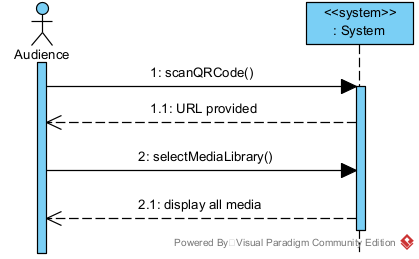
\includegraphics[width=0.8\textwidth]{images/SSD-UC01-ViewMediaLibrary.png}
    \centering
    \caption{System Sequence Diagram: View Media Library}
\end{figure}

\textbf{Operation:} selectMediaLibrary() \\
\textbf{Cross-References:} UC01 (View Media Library) \\
\textbf{Pre-conditions:}
\begin{itemize}
    \item Media items, \emph{m}, exists in system
    \item \emph{m} is approved for view
\end{itemize}
\textbf{Post-conditions: }
\begin{itemize}
    \item List of media, \emph{ml}, is created
    \item \emph{ml} is returned to user
\end{itemize}
